\hypertarget{introduction}{%
\section{Introduction}\label{introduction2}}

The motivation of this thesis is twofold: firstly, to create
three-dimensional epithelia with controlled pressure, and secondly, to
study the material response of the tissue to different regimes of
tension. To achieve the first objective, we have developed a monolayer
inflator (MOLI) device that allows us to fabricate epithelial domes
where cells can be stretched to more than 100\% of area strain.

Epithelial tissue plays a crucial role in various physiological
functions, and must therefore undergo deformation over a wide range of
timescales and magnitudes. Similarly, pressure levels also vary widely
in different contexts. For instance, the luminal pressure in blastocysts
doubles over the course of its development, resulting in changes in
cortical tension and strain. The MDCK dome system provides a suitable
platform to investigate the interplay between cell strain, tension, and
pressure. Previous studies by Latorre et al.~have observed a wide range
of pressure throughout the evolution of the dome, and cells have
exhibited a range of deformation, including active-superelastic
behavior. However, the control in this system is limited to the
footprint of the domes. In this chapter, we aim to utilize the MOLI
system to subject tissues to a range of strain and tension regimes.
\hypertarget{measurement-of-dome-mechanics}{%
	\section{Measurement of dome
		mechanics}\label{measurement-of-dome-mechanics}}

To measure the kinematics of the domes, we analyzed the midsection of
the domes, assuming symmetry of spherical caps. We measured the height
\(h\) and base radius \(a\). This allowed us to calculate the radius of
curvature \(R\) using trigonometry. \[ R = \frac{h^2 + a^2}{2h} \] This
also allowed us to compute the tension \(\sigma\), given by Laplace's
law. \[\sigma = \frac{\Delta PR }{2}\] For the dome strain, we used the
areal strain measure, which is computed based on the surface area. We
compared the dome surface area to the area of the footprint.

\begin{figure}
	\begin{minipage}[c]{0.7\textwidth}
		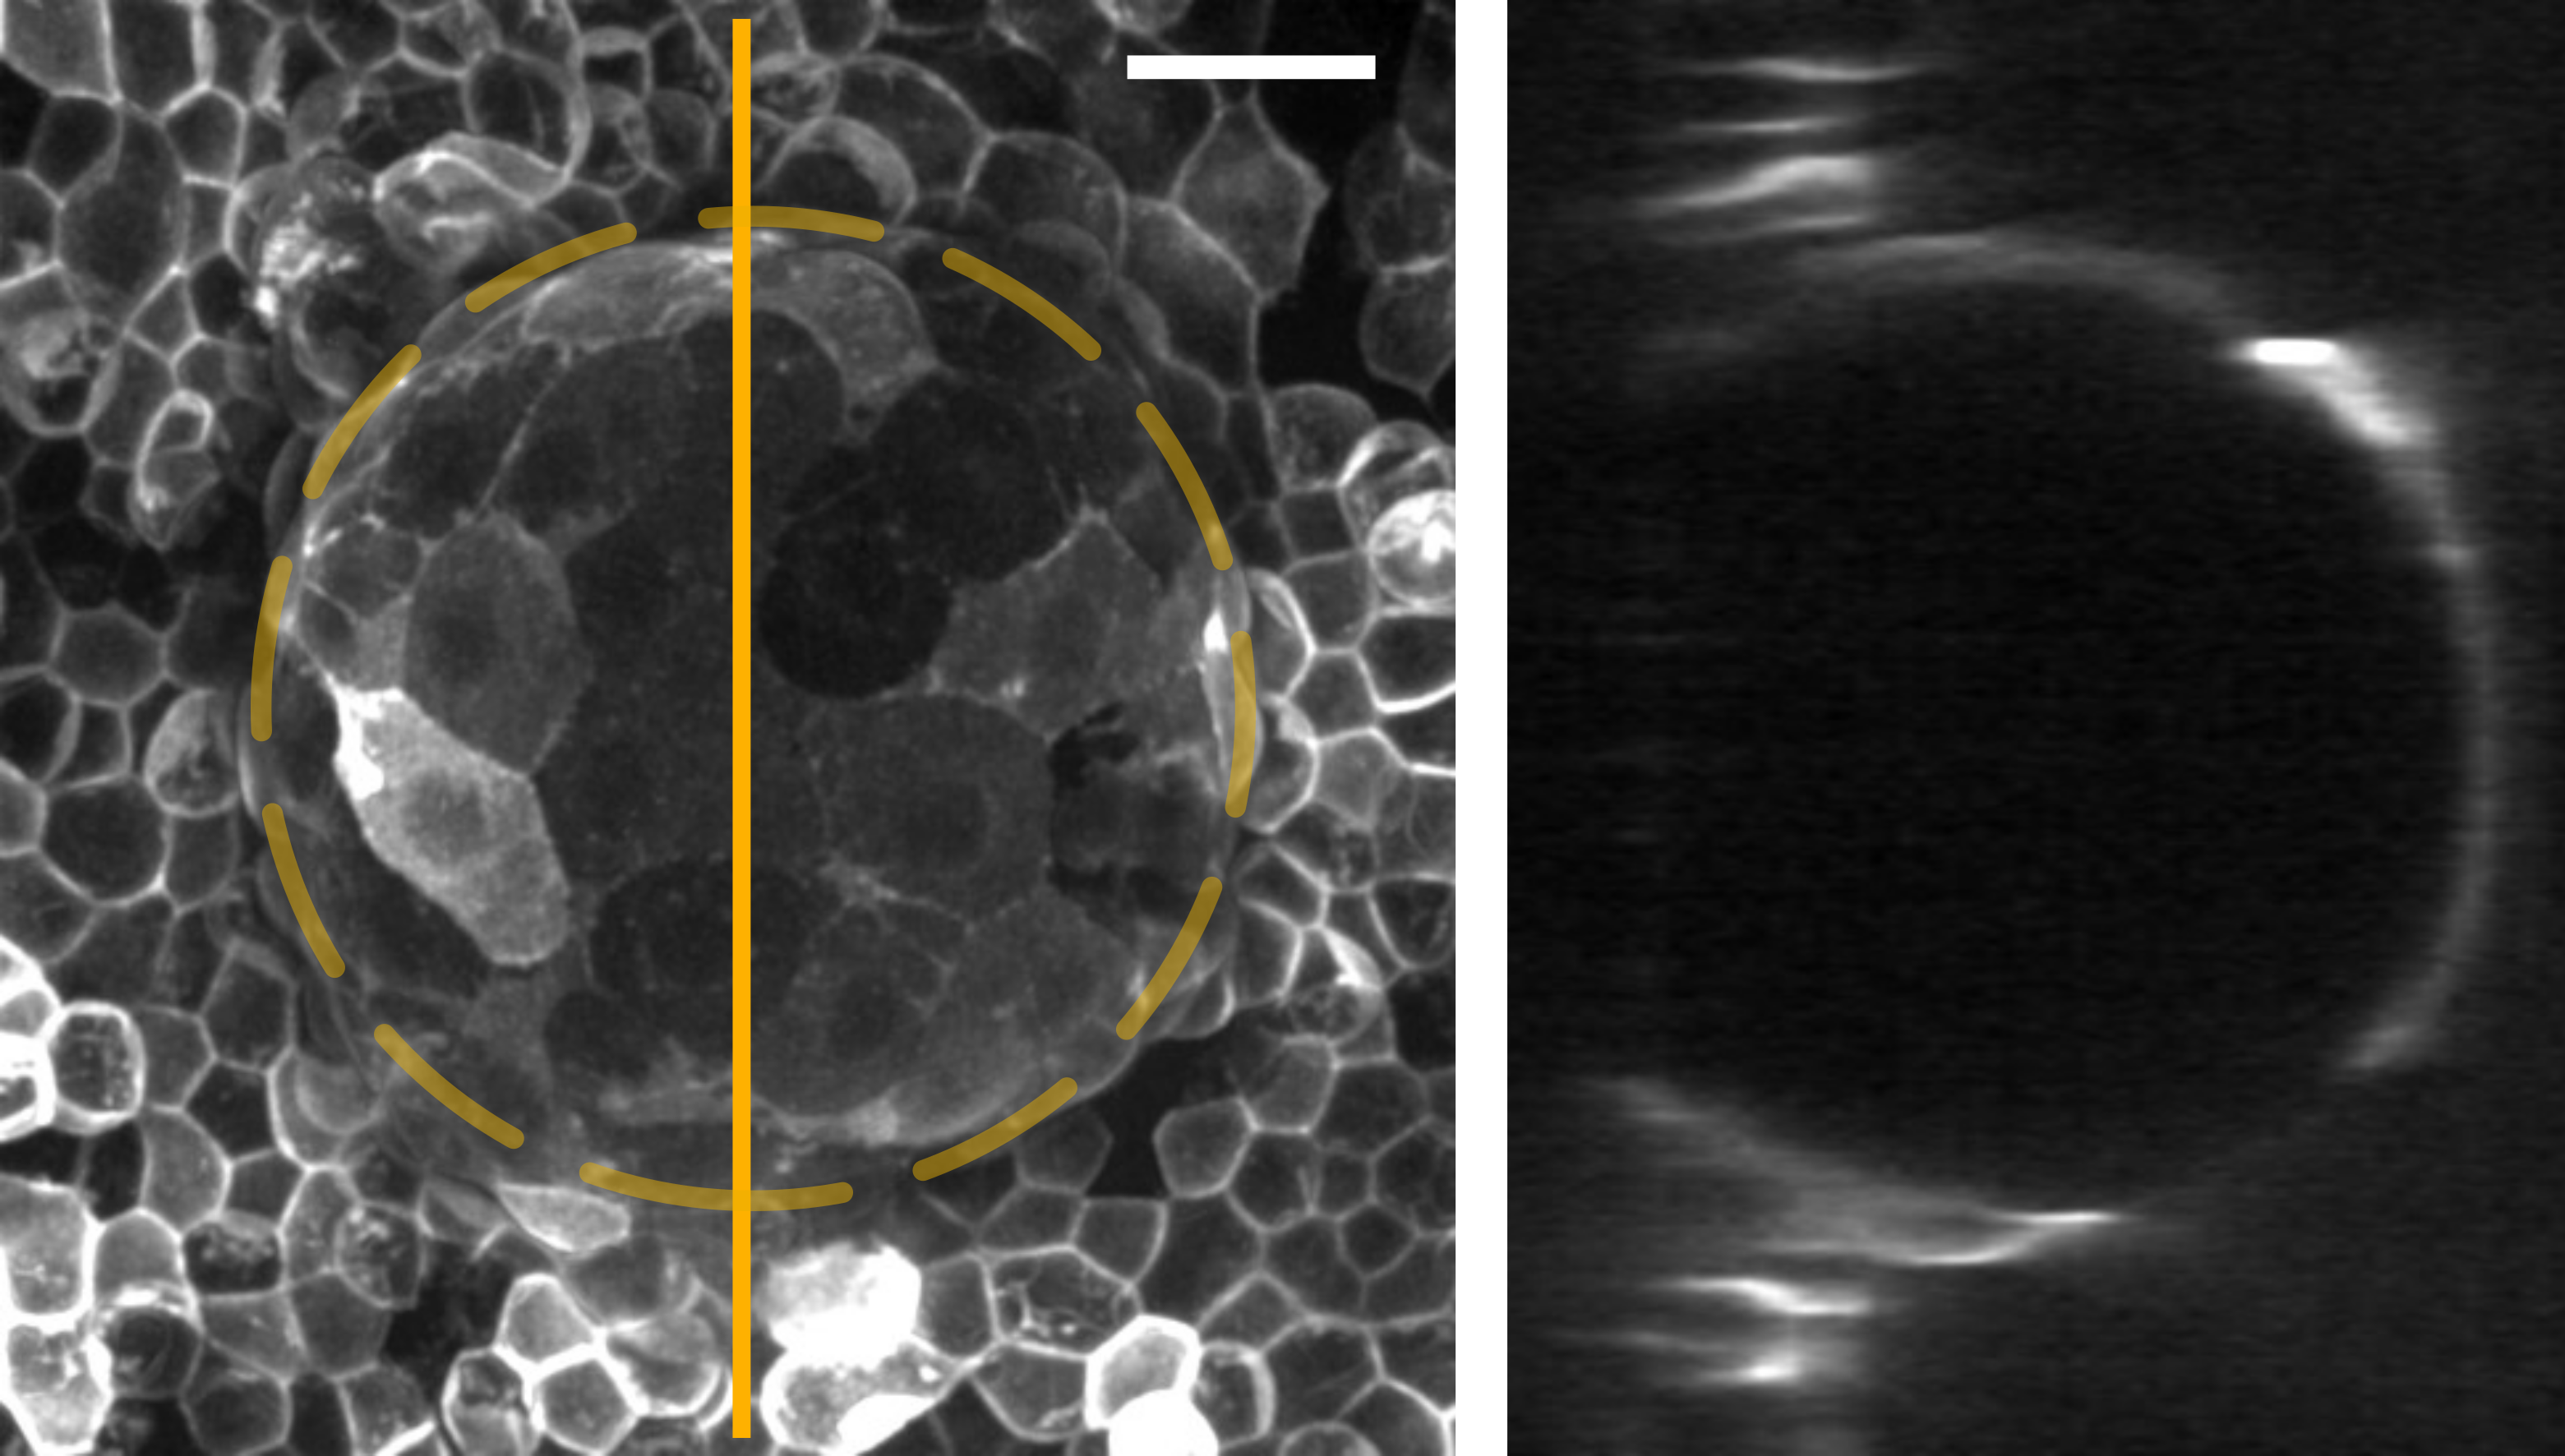
\includegraphics[width=\textwidth]{chap7_realdome.png}
	\end{minipage}\hfill
	\begin{minipage}[c]{0.27\textwidth}
		\caption{\\ \textbf{Spherical cap}:\\Here is an example of an epithelial dome at 200 Pa, which has increased its surface area four times the original footprint. One can clearly appreciate the beautiful spherical shape of the dome in the cross-section. Scale bar is $20 \mu m$.
		} \label{fig_7_1}
	\end{minipage}
\end{figure}


\[ \epsilon = \frac{A_{dome } - A_{footprint}}{A_{footprint}} \]
\[ \epsilon = \frac{\pi(h^2 + a^2) - \pi a^2}{\pi a^2} = \frac{h^2}{a^2}\]
Using the line scan method of imaging domes for fast time-lapse, we
obtained a large number of frames for the analysis of the height and
radius of curvature. Thus, we used kymographs of the top section of the
dome. Kymographs are images with a cross-section of the dome top with
respect to time. Using image processing MATLAB code, we obtained the
location of the maximum intensity value for a particular time in the
graph to obtain the time evolution of the height of the dome. The same
method was used for the base radius as well. The kymograph of the base
radius allowed us to keep track of delamination, as it could change the
value of strain.

\hypertarget{epithelial-domes-at-constant-pressure}{%
	\section{Epithelial domes at constant
		pressure}\label{epithelial-domes-at-constant-pressure}}

Initially, our focus was to investigate the behavior of domes under
constant pressure. We conducted experiments inflating domes at varying
pressures, but observed that hardly any of the domes formed at pressures
lower than \(50-100 Pa\). After optimizing for different pressures, we
settled on using \(200 Pa\) which allowed domes to form without
delaminating out of pattern.

\begin{figure}
	\centering
	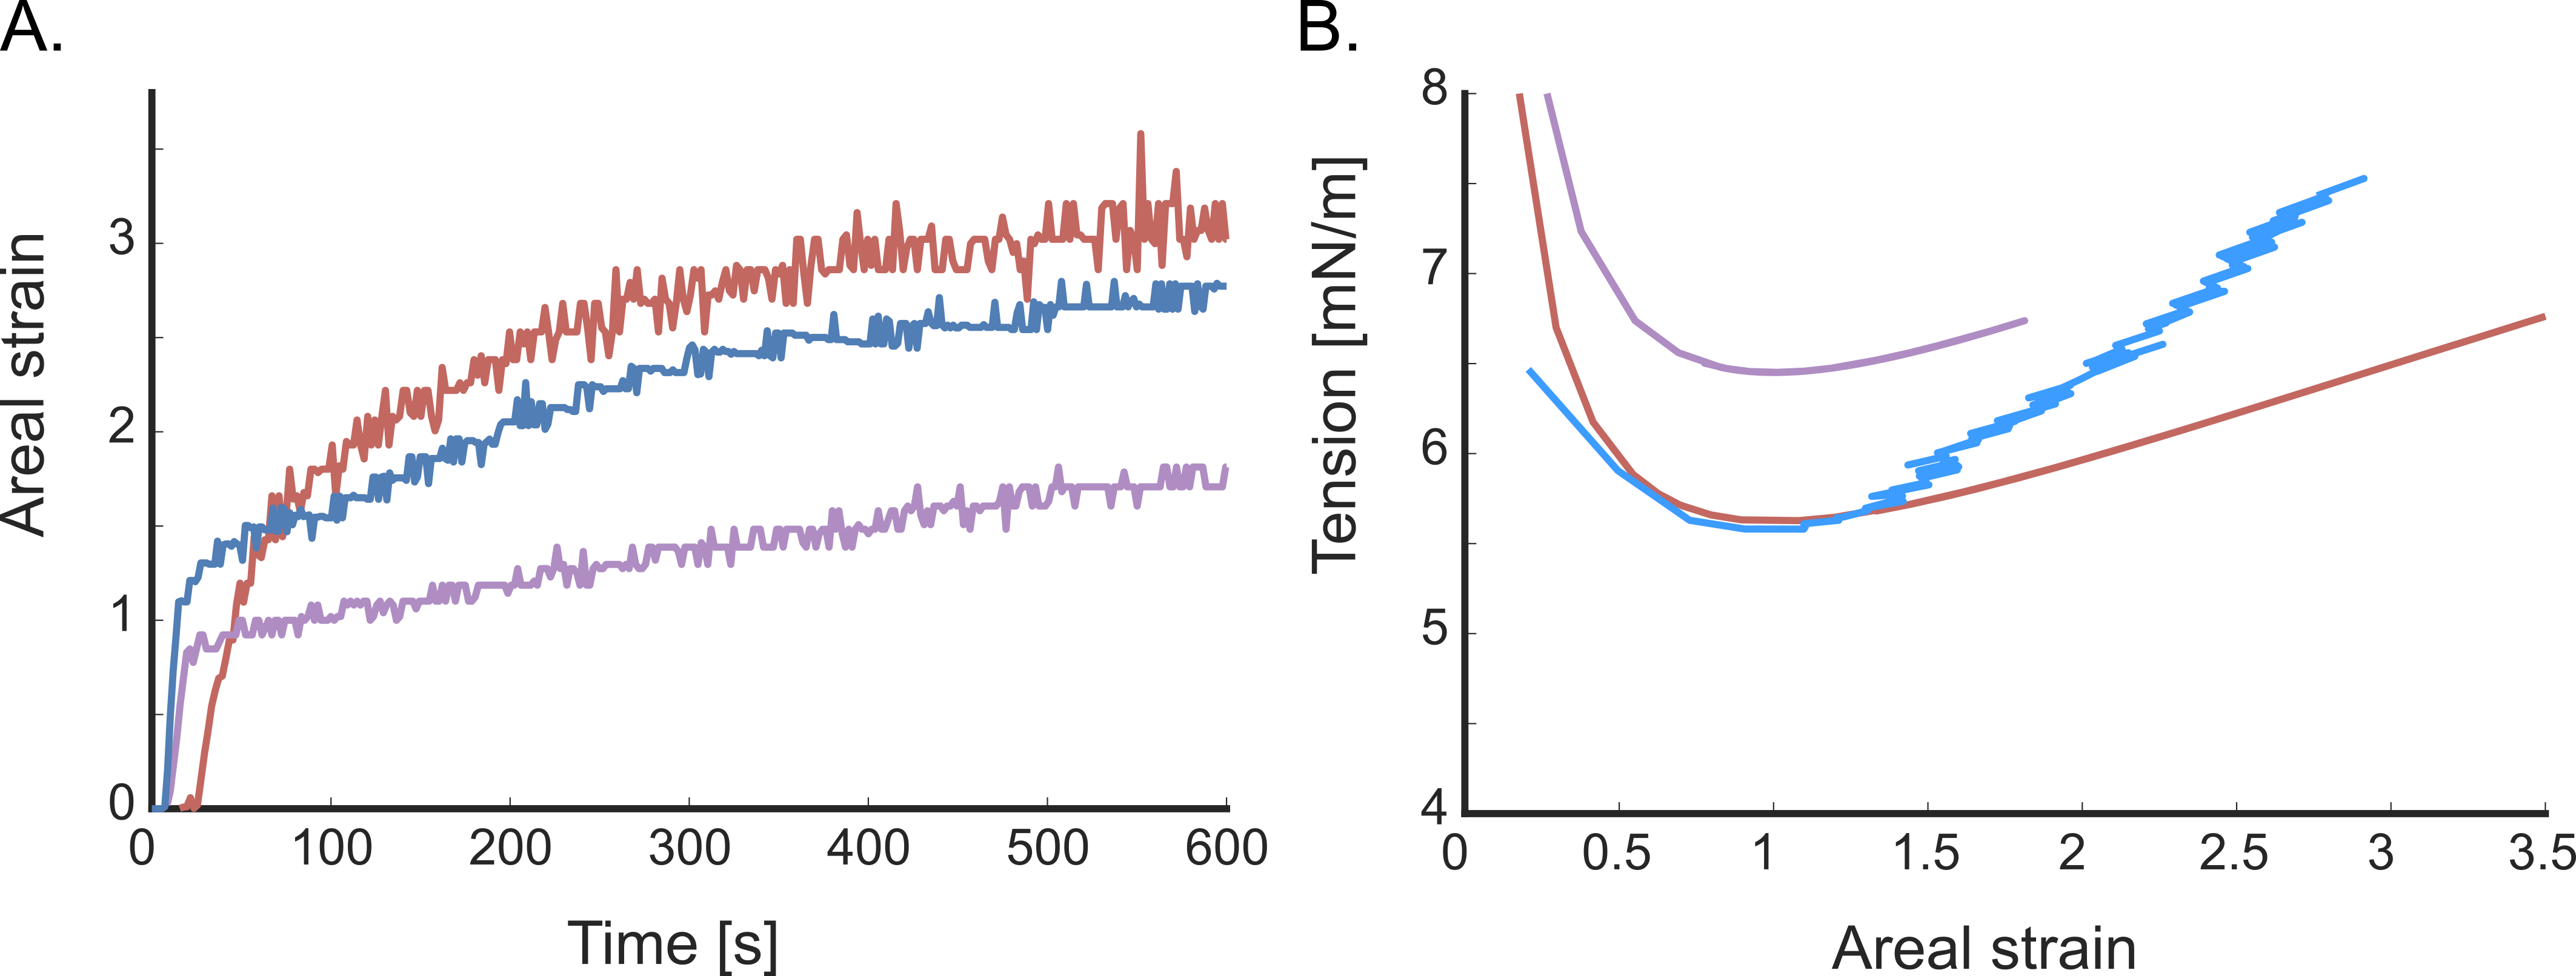
\includegraphics[width=\textwidth]{chap7_constpressure.png}
	\caption{\label{fig_7_3} \textbf{Epithelial domes at constant pressure}: Dynamic response of the representative domes at constant pressure of 200 Pa (A) Areal strain vs time. (B) Tension vs areal strain (Nike curves).
	}
\end{figure}

Our results indicate that the areal strain of the dome increases during
the first \(3-5\) minutes of pressure application, and then reaches a
plateau in strain until \(5-10\) minutes. Despite large dome-to-dome
variability, with strains ranging from \(50\%\) to \(300\%\), the
stabilization in strain suggests that a steady state has been achieved
by the tissue.

Further examination of the tension-strain relationship of these domes
revealed a distinctive curve, resembling the swish symbol of ``Nike''.
The tension is extremely high for low strains, and then decreases to a
minimum around an areal strain of one, where the dome forms a perfect
hemisphere. The tension increases again, but the slope is relatively
gentle as compared to the steep decline observed at low strains.

This kind of material response would be unusual for typical materials
undergoing biaxial stretching. However, in our case, the underlying
cause of this curve can be attributed to the geometric constraint
imposed by the dome system and force balance (Laplace's law). Since the
tension in the dome is a function of its radius of curvature, the radius
of curvature starts out very high, producing higher tension that then
reduces to a minimum with a hemispherical shape before increasing again.
The radius of curvature, areal strain, and tension are inherently
interconnected, such that at a constant pressure, we can write the
expression of the curve as:

\[ R = \frac{h^2 + a^2}{2h} \] \[ R = \frac{h^2/a^2 - 1}{2h/a^2} \]
\[ R = a\frac{\epsilon^2 - 1}{2\sqrt{\epsilon}} \]
\[ \sigma = \frac{Pa}{4} \frac{\epsilon^2 - 1}{\sqrt{\epsilon}}\]

Normalizing the tension with the base radius results in all domes
collapsing onto one curve corresponding to a specific pressure. We call
this curve the ``isobaric'' curve.

In terms of physics, we understand that when the step pressure is
applied, the dome suddenly inflates and has to undergo non-steady state
out-of-equilibrium stresses. It is clear that this curve does not
represent the quasi-static constitutive relation of the epithelial
tissue.

\begin{figure}
	\centering
	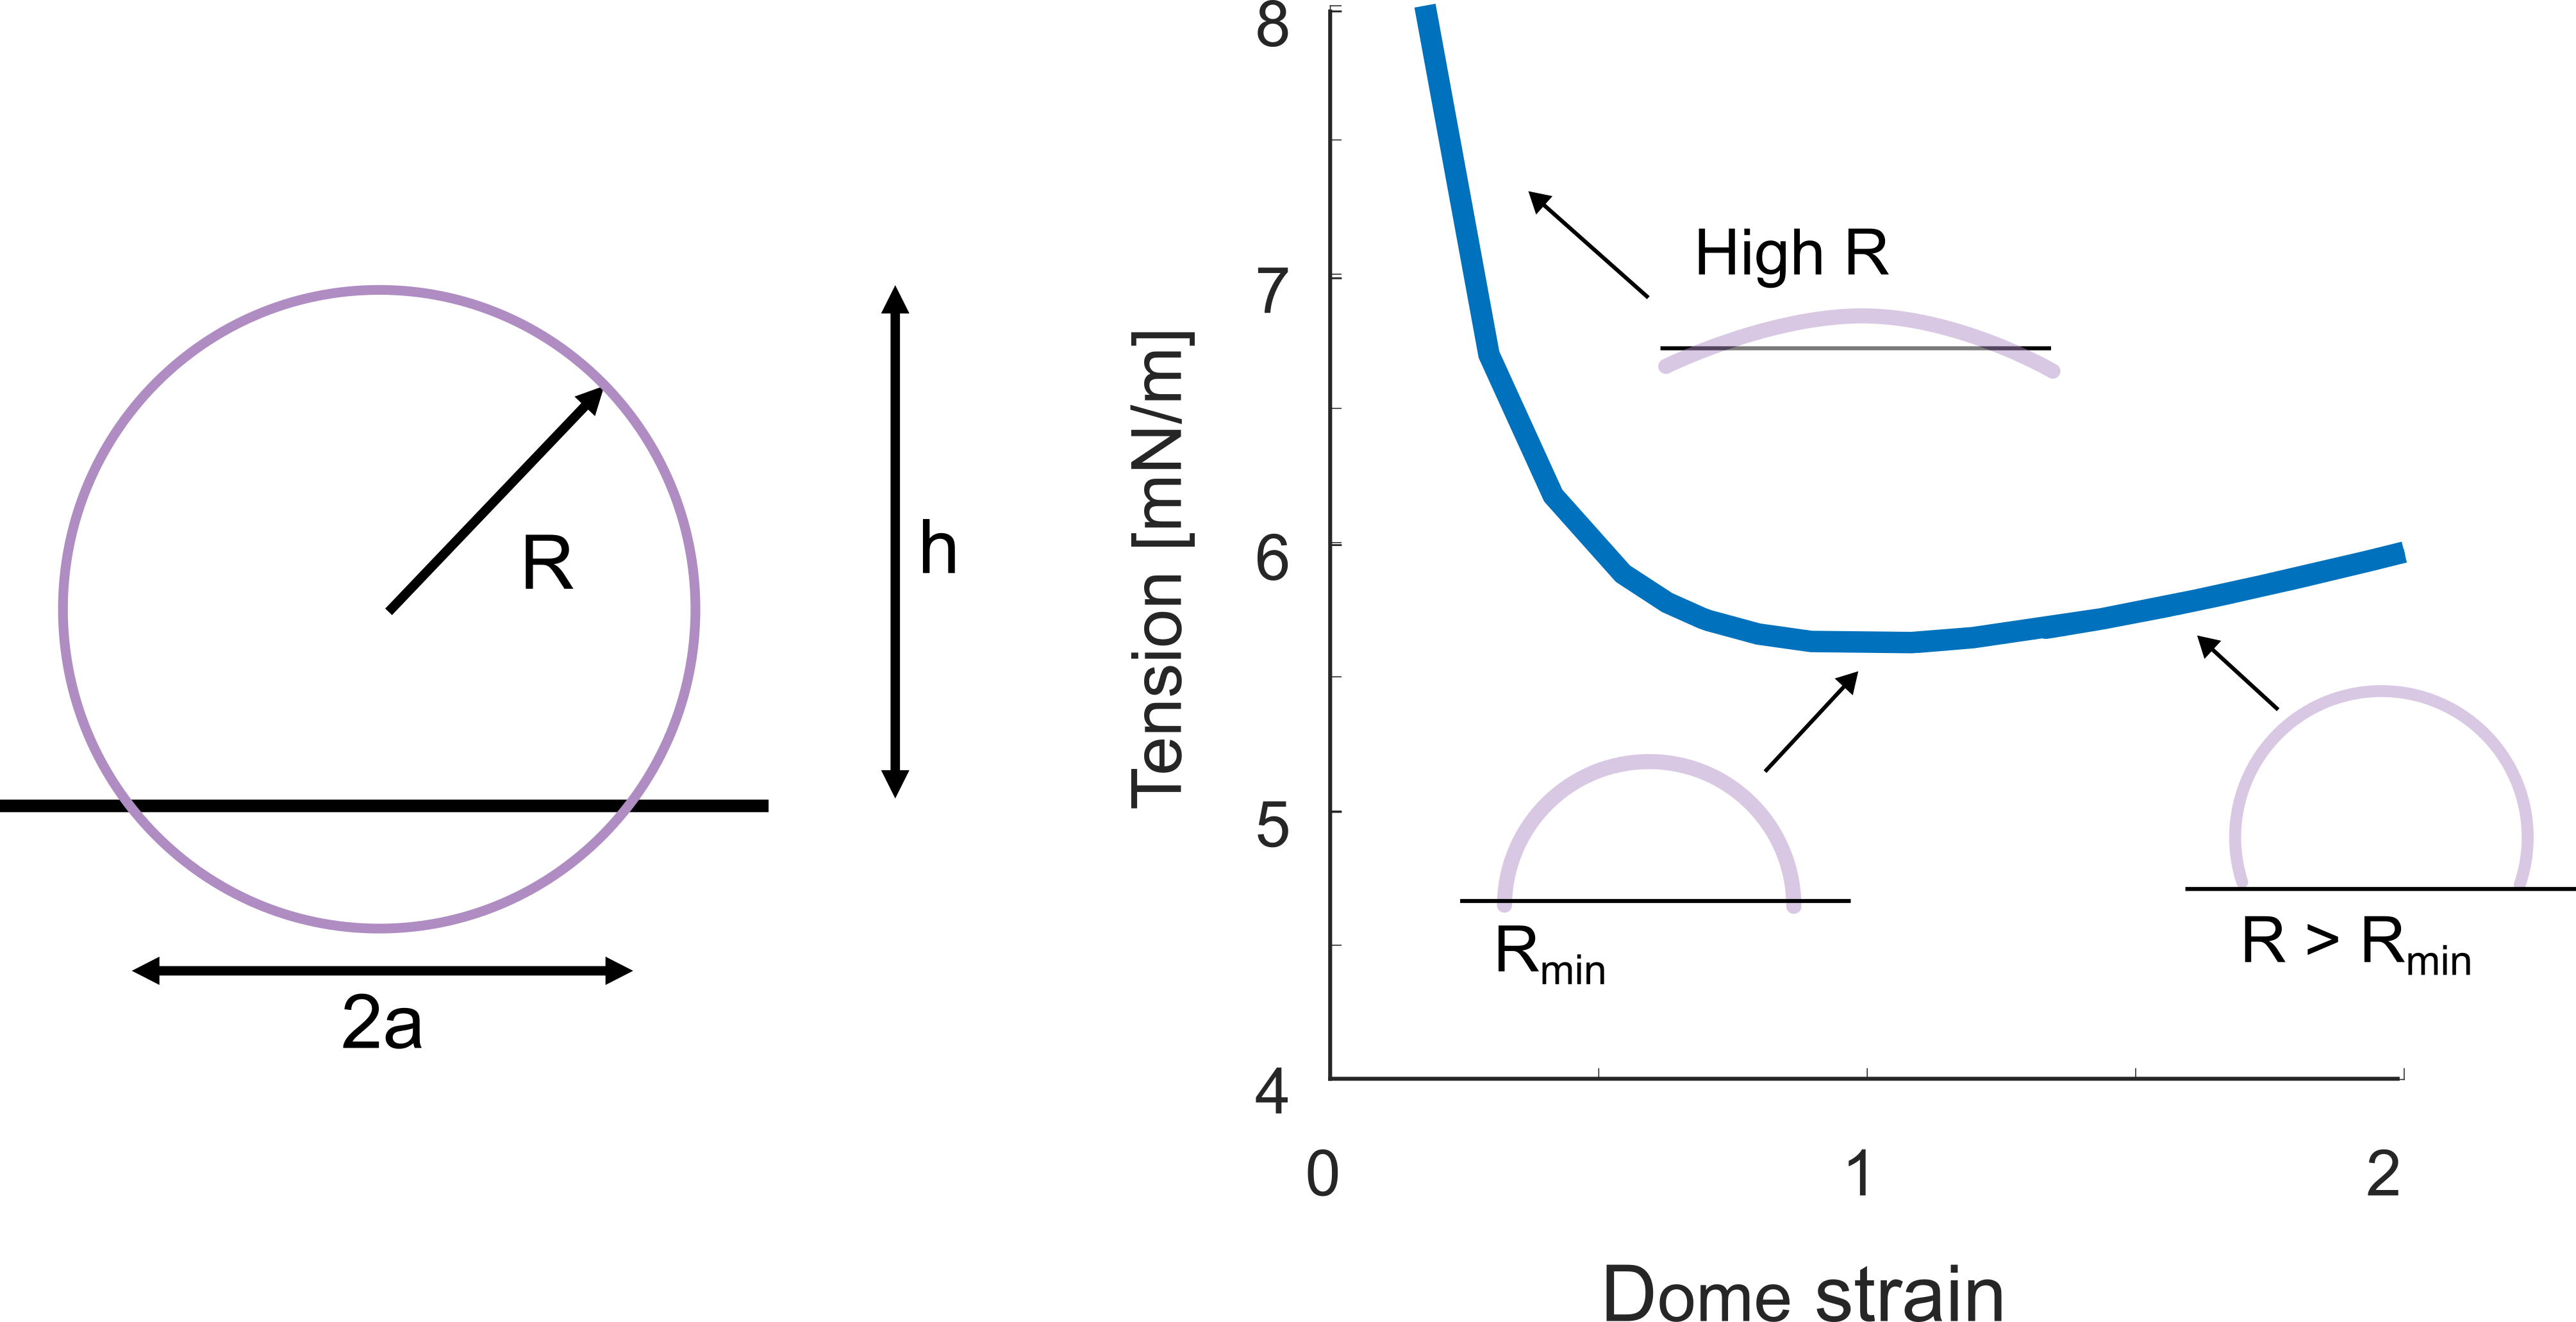
\includegraphics[width=0.8\textwidth]{chap7_radius.png}
	\caption{\label{fig_7_4} \textbf{Explanation for isobaric curve}: Tension and strain are related to each other through geometric constraint of spherical cap.
	}
\end{figure}



\hypertarget{constitutive-relation-of-epithelia}{%
	\section{Constitutive relation of
		epithelia}\label{constitutive-relation-of-epithelia}}

In order to obtain the actual constitutive relation, it is ideal to
increase strain or tension in a quasi-static manner. However, in our
system, we are only able to control pressure. Slowly increasing pressure
is not feasible with domes because they do not delaminate at low
pressures. If they do, they are in a non-steady state regime where they
quickly inflate to higher strains. As a result, we chose to capture
steady states corresponding to different pressures.

We applied a pressure of 200 Pa for 5 minutes until the dome reached a
steady state. Then, we reduced the pressure by 20 Pa and waited for the
dome to reach a steady state again. We repeated this process until the
dome was completely deflated. In this way, the tension-strain curves
captured parts of different isobarics as the dome passed through
different pressure steady states.

We obtained a constitutive relation that exhibits a initial increase in
tension with strain for lower strains. However, for larger strains, the
tension seems to plateau consistently with earlier studies of MDCK
domes. It is worth noting that the variability in dome-to-dome tension
is significant, and the tensions recorded of 4.5 mN/m are of the same
order of magnitude as in previous studies.

\begin{figure}
	\centering
	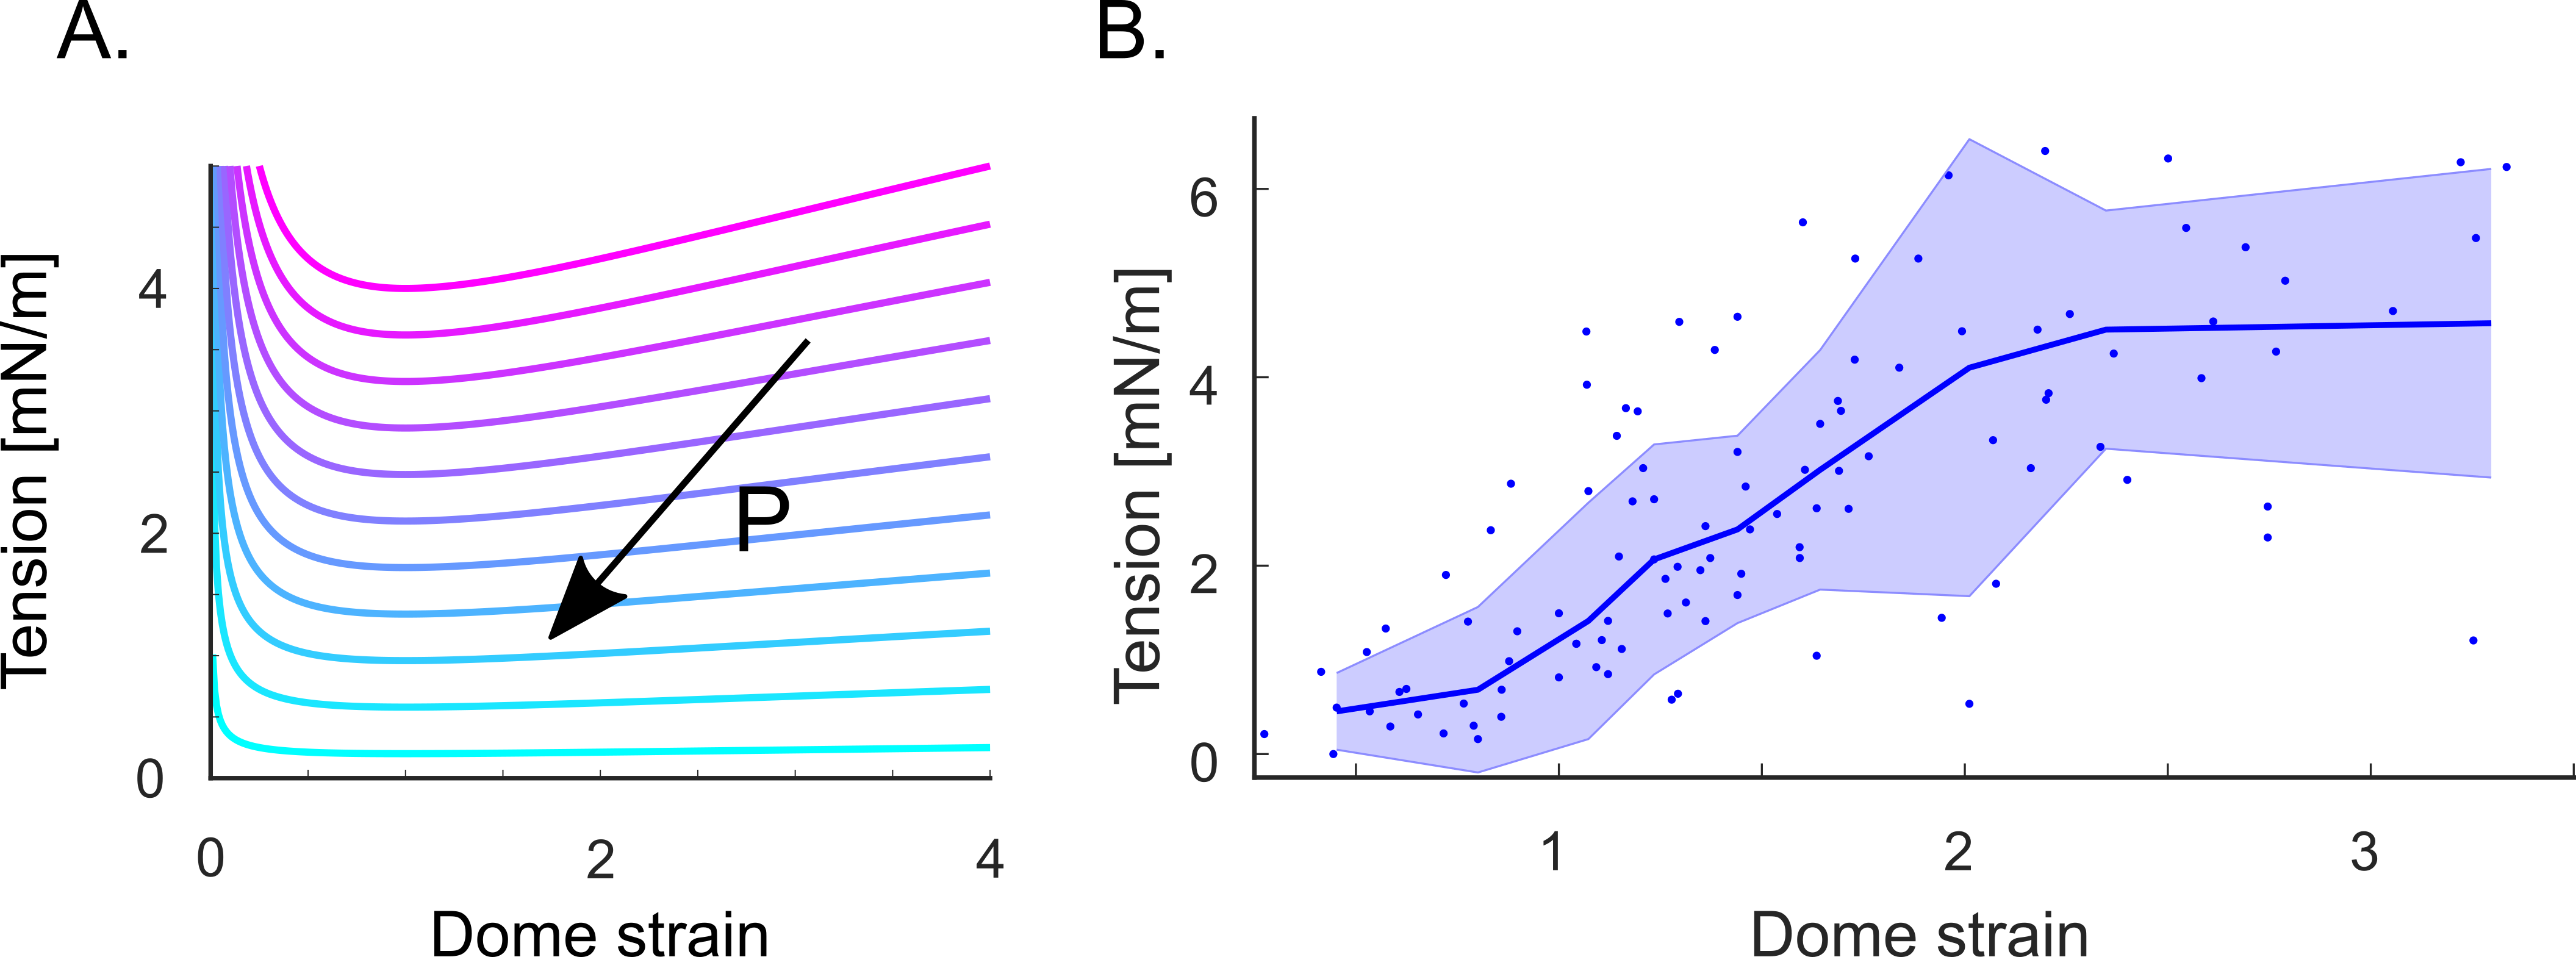
\includegraphics[width=\textwidth]{chap7_constitutivelaw.png}
	\caption{\label{fig_7_5} \textbf{Constitutive Relation of Epithelia}: (A) We will set up experiments to probe the steady state at different pressures. We will start from the highest pressure, move along the isobaric line and achieve a steady state, and then move down to the next isobaric line, and so on.	(B) The constitutive relation between dome strain and tissue tension was experimentally obtained (n=12). The line and shaded area represent the median and standard deviation, respectively, by binning 13 points in each bin.
	}
\end{figure}


\hypertarget{dynamics-of-the-epithelia-domes}{%
	\section{Dynamics of the epithelia
		domes}\label{dynamics-of-the-epithelia-domes}}

Table1: Time period: 6s 60s 600s Rates: 0.2Pa/s 1.5Pa/s 20Pa/s

To investigate the dynamic material response of the domes, we conducted
cyclic stretching experiments by subjecting them to a triangular wave of
pressure with a magnitude of 200 Pa at three different timescales. Based
on the literature on cell remodeling and experimental conditions, we
chose cycles of 20 s, 266 s, and 2000 s.

\begin{figure}
	\centering
	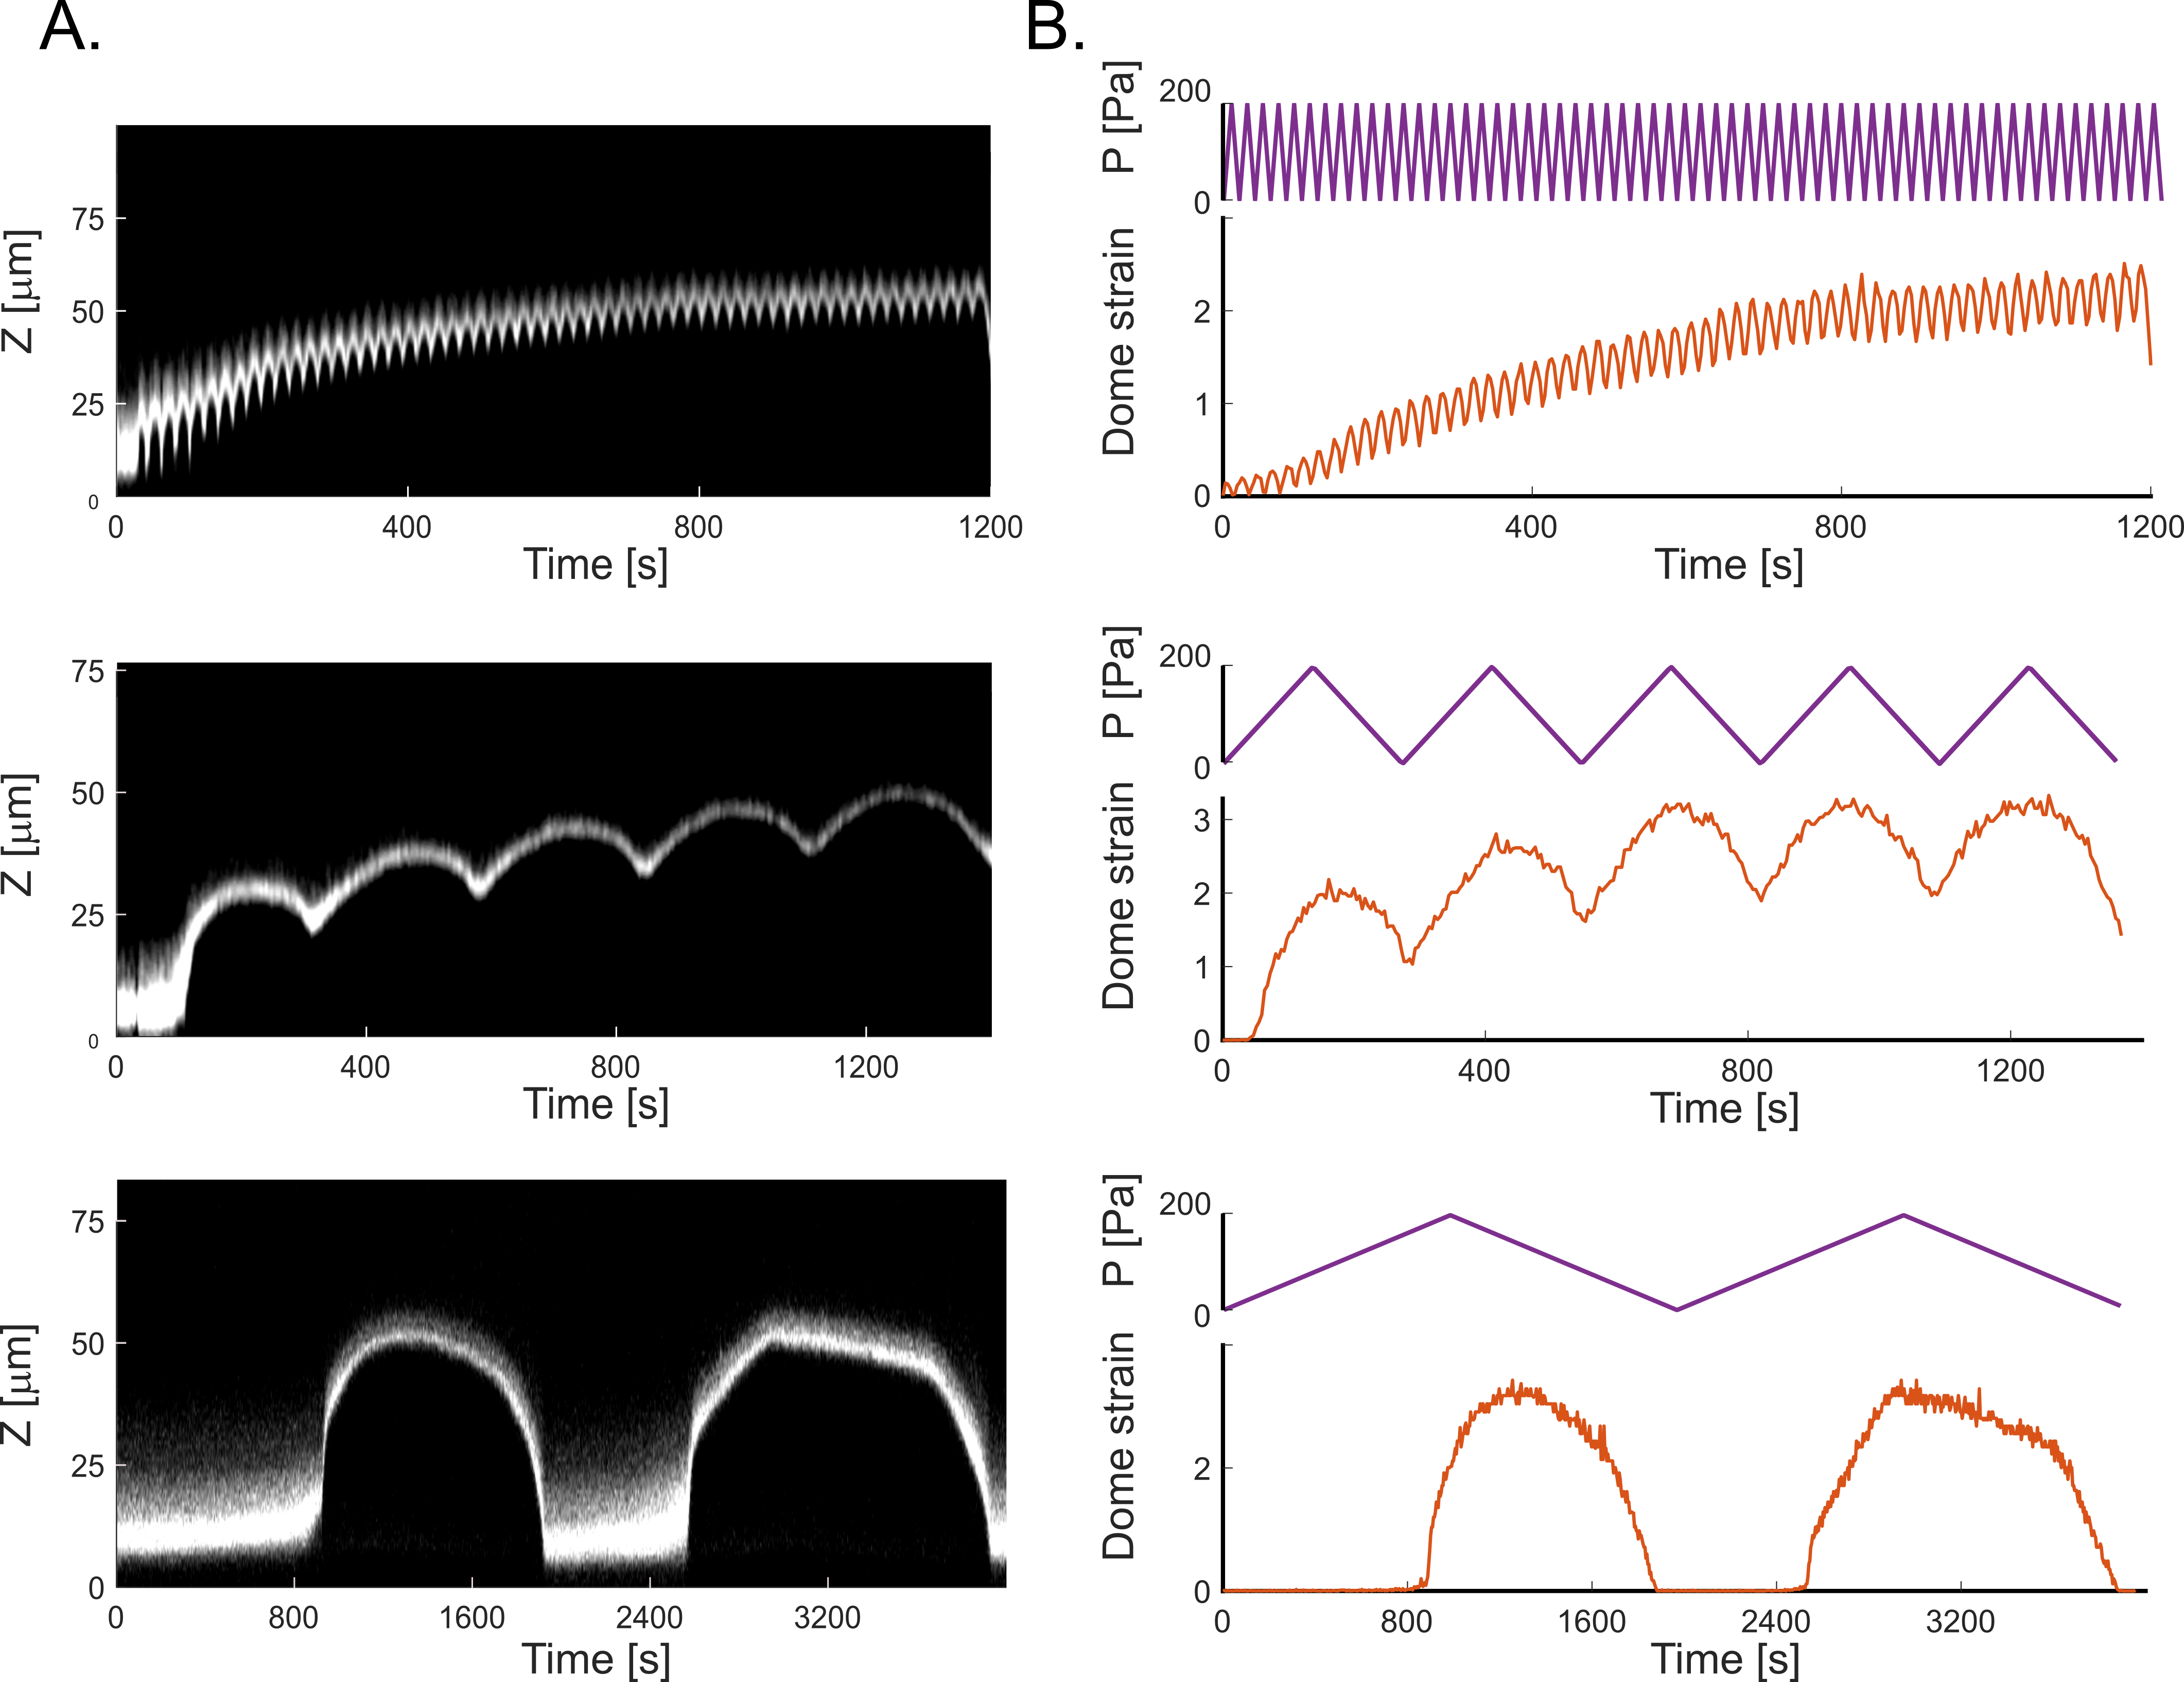
\includegraphics[width=\textwidth]{chap7_dynamic.png}
	\caption{\label{fig_7_6} \textbf{Dynamic response of Epithelia:} (A) The XZ plane images and kymographs of domes subjected to cyclic pressure between 0 to 200 Pa with rates of 20, 1.5, and 0.2 Pa/s The kymographs generated along the midsection of the domes indicated by yellow dotted lines. These indicate the evolution of height of the domes with respect to time. (B) The strain response of domes to cyclic pressure with different rates. Magenta represents pressure and red represents strain with respect to time. For A, B, n= 7 domes for 20 Pa/s, n = 8 for 1.5 Pa/s, and n = 7 for 0.2 Pa/s. 
	}
\end{figure}


In the case of the fastest cycles, we observed that the domes
progressively stretched more as the cycles progressed until they reached
a steady state oscillation. We conducted the experiment for 1200 s (60
cycles) and noticed that the domes accumulated strain progressively.
While loading, they stretched, and while unloading, they unstretched but
did not return to zero strain after the first few cycles. In the last
few cycles, we observed that the dome oscillated between two states of
strains.

A similar response was observed for the moderate cycles, where the domes
were stretched for five cycles of 266 s each. The strain accumulated in
the first cycle itself, with strains reaching higher values than those
observed in the fast case. Additionally, after a few cycles, the dome
appeared to have reached a steady state.

For the slowest cycles of 2000 s, we faced difficulty in forming domes
at lower pressures. As previously mentioned, the domes did not detach
until they reached a critical pressure of 100-150 Pa, after which they
rapidly inflated to high strains of 200-300\%. However, it was evident
that the strains did not accumulate, and there was no difference in the
maximum strains achieved in both cycles, indicating that the steady
state was reached immediately at this timescale.

One puzzling observation was that in some cases of moderately fast
cycles, there was a delayed peak in strain compared to the maximum point
of pressure, indicating that when the pressure reduced, the dome
continued to inflate and increase the strain.

\hypertarget{active-gel-tissue-model}{%
	\section{Active gel tissue model}\label{active-gel-tissue-model}}

In addition, to complement our experimental findings, we collaborated
with Adam Ouzeri to develop a computational framework. Our understanding
of epithelial mechanics suggests that the viscoelasticity of the actin
cortex plays a crucial role in sustaining deformations at the timescale
of seconds to minutes. Adam Ouzeri developed a theoretical framework
that bridges active gel models of the actomyosin cortex and 3D vertex
models at tissue scales. In this model, each cell is represented by an
active gel surface that accounts for the physical aspects of the cortex,
and a tissue is assembled from a collection of these active gel
surfaces. The dynamics of the system are formulated through a balance of
different potentials that represent different active internal or
external forces and dissipation.

The framework accounts for the molecular dynamics of the actin filament
network, myosin, and crosslinker proteins through four main components:

\begin{figure}
	\centering
	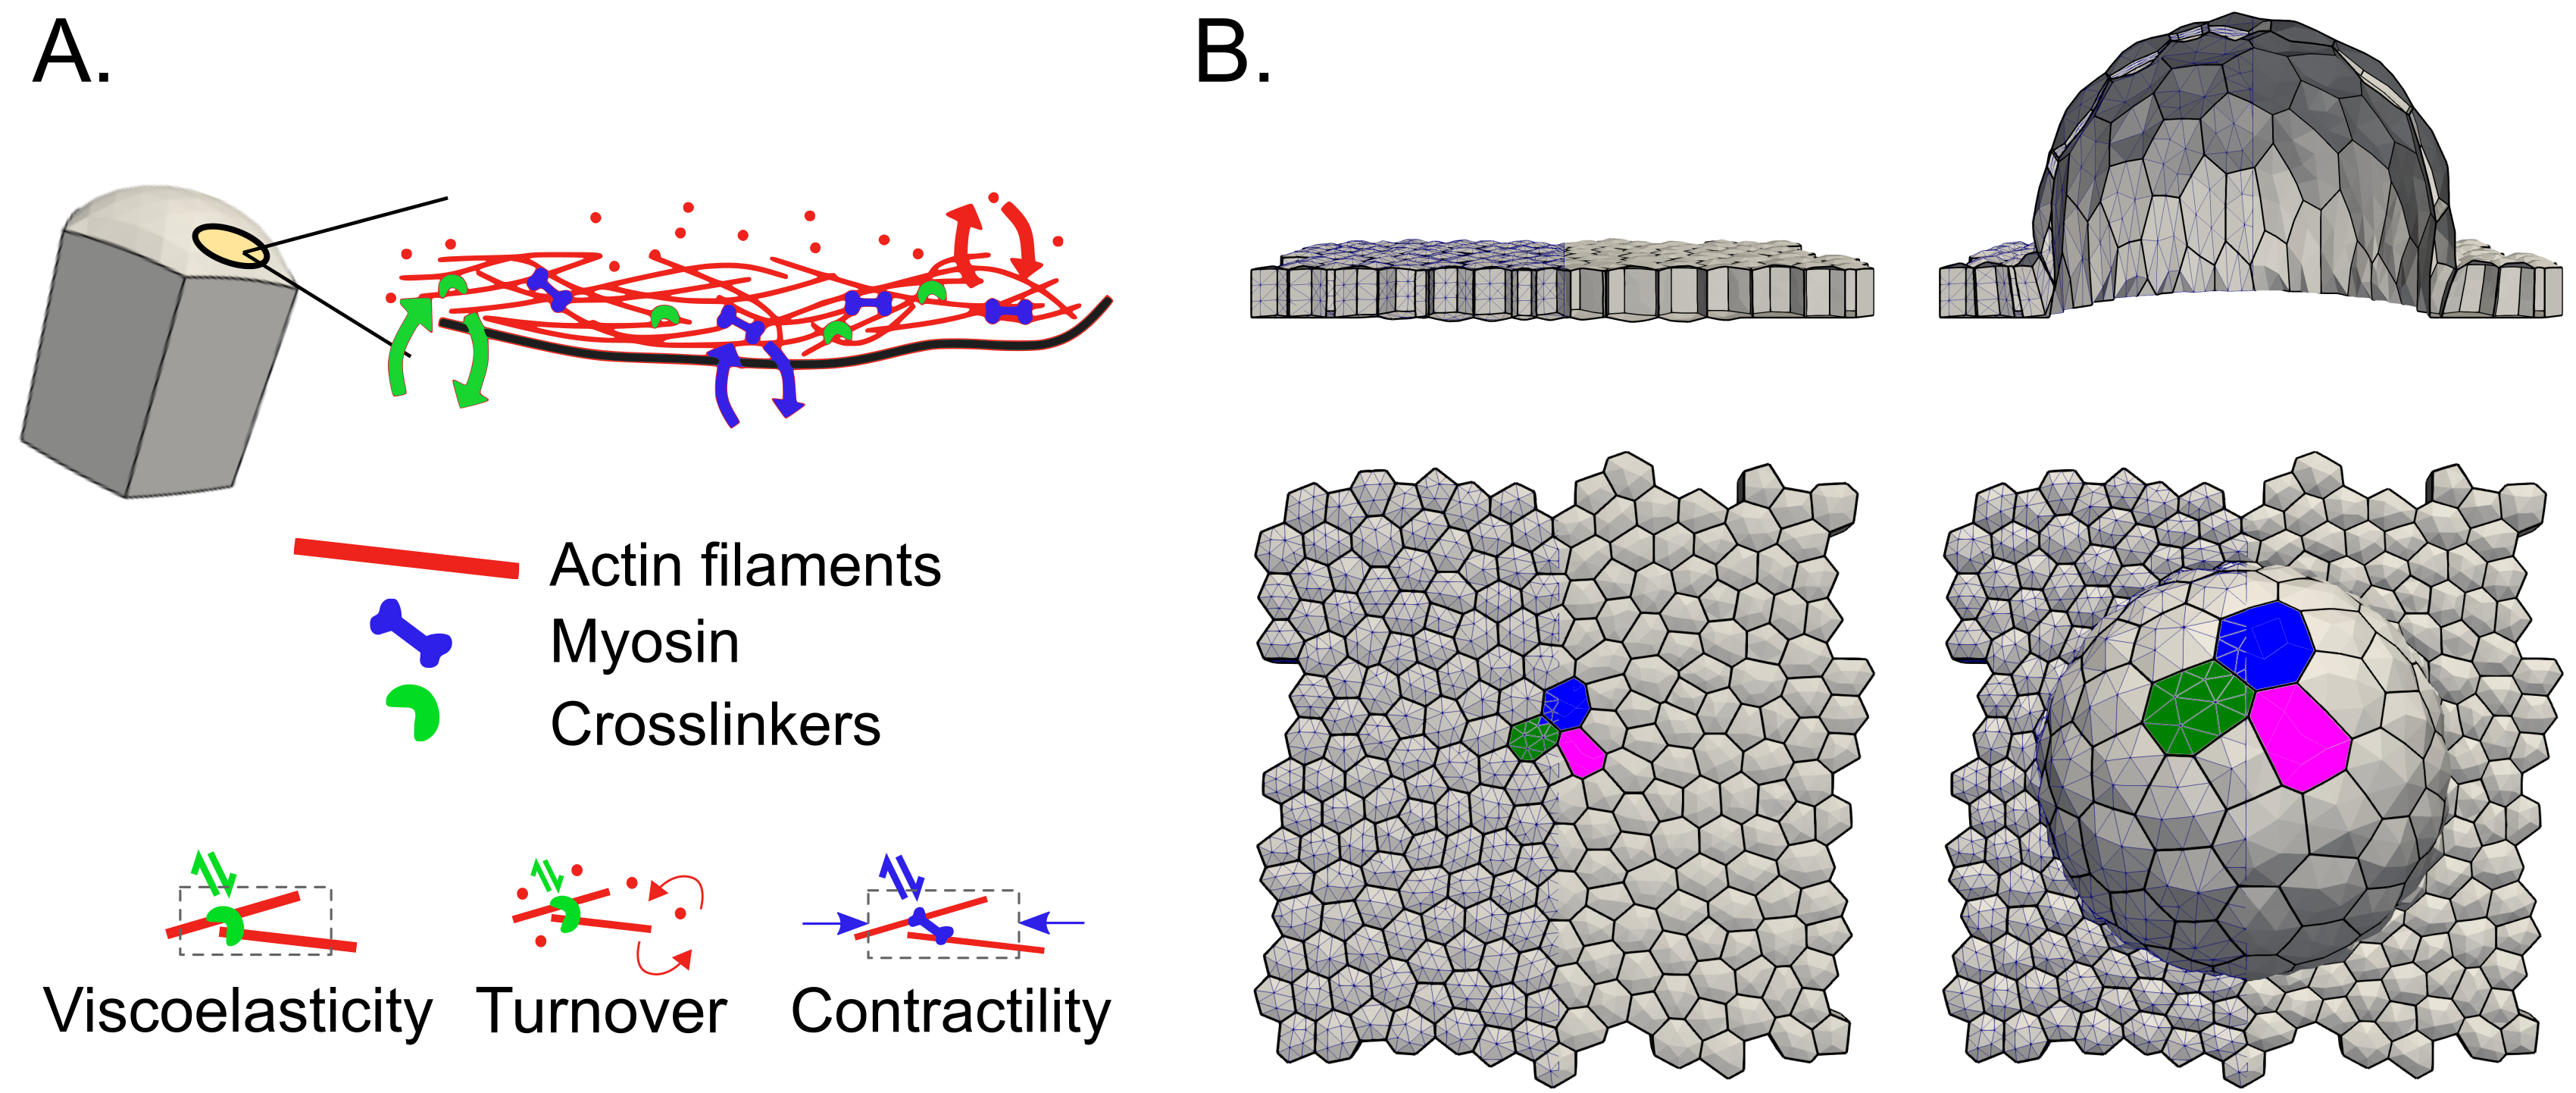
\includegraphics[width=\textwidth]{chap7_digitaldome.png}
	\caption{\label{fig_7_2} \textbf{Stress strain behavior of materials}: (A) materials being stretched or compressed. (B) Quasistatic deformations yield stress-strain curves. (C) Creep test where strain response is characterized at constant stress.
	}
\end{figure}

\begin{enumerate}
	\def\labelenumi{\arabic{enumi}.}
	\item
	\textbf{Cortical thickness:} The cell cortex is modeled as a
	hyperelastic membrane with cortical thickness (\(\rho_R\)). The
	deformation kinematics of this model is defined by mapping a cortical
	patch from a reference configuration \(\Gamma_0\) to a deformed
	configuration \(\Gamma\) with metric tensor \(G_0\) to \(g\),
	respectively. As the material is dynamic, the reference configuration
	has to be dynamic as well. Thus, there is a second reference
	configuration with a dynamic metric tensor \(G\). The cortical
	thickness in the reference configuration changes with the mapping
	change represented by the Jacobian \(J_R\). This is expressed as
	\(\rho_R(\xi, t) = \rho(x,t)J_R(\xi,t)\).
	\item
	\textbf{Network elasticity:} This potential accounts for the free
	energy of the system undergoing deformation. The potential is
	dependent on the difference between in-plane strain (\(C\)) and the
	metric (\(G\)) written in the format of a hyperelastic potential
	(\(W\)). Using a Neo-Hookean elastic potential, \(W\) depends on two
	Lamé parameters, \(\lambda\) and \(\mu\). This potential is expressed
	as \(\mathcal{F} = \int_{\Gamma_R} \rho_R \ W(\mathbf{C,G})dS_R\).
	\item
	\textbf{Dissipation:} The actomyosin network remodels under tension,
	and the released elastic energy can be accounted for with a
	dissipation potential. The potential depends on a coefficient \(\eta\)
	equivalent to bulk viscosity, cortical thickness, and the rate of
	metric tensor given by \(\dot{G}\). This potential is expressed as
	\(\mathcal{D} = \int_{\Gamma_R} \frac{\eta}{2}\ \rho_R \ \mathbf{\dot{G}}:\mathbf{\dot{G}} \ dS_R\).
	\item
	\textbf{Active contractility:} The model is an active gel, and the
	active part is included through an active power potential that adds
	energy to the system. The potential is dependent on the cortical
	tension and the rate of deformation tensor. The cortical tension is an
	active tension component of the network that is proportional to
	cortical thickness. This potential is expressed as
	\(\gamma(\rho) = \rho \xi\) and
	\(\mathcal{P} = \int_{\Gamma} \gamma : \mathbf{d} \ dS\).
\end{enumerate}

Additionally, we account for turnover dynamics in the cortex through a
mass balance law. Here, we assume that there is a steady-state cortical
thickness, and the network is constantly polymerizing and depolymerizing
with cytosolic components. This is expressed as
\(\dot{\rho} + \rho \ tr(\mathbf{d}) = k_p\ C - k_d\ \rho\).

The proposed governing equations are obtained by minimizing the
Rayleighian, which is given as:

\[ \mathcal{R} = \frac{dF}{dt} - D + P + P_e \]


%\begin{center}
%	\begin{mybox}{gray}{  \center{\label{A} \textbf{ Box A: Governing equations for a 2D compressible active nematic gel}}}
%		
%		\textbf{Constitutive relations}
%		\newline
%		Power conjugate to the rate of deformation tensor $d_{ab}$ is given as
%		\begin{align}  \label{eq_box_A_2}
%			& \sigma^{\rm s}_{ab} = \rho \left[2\eta  (d_{ab}+d_{cc} \delta_{ab}) + \beta  \widehat{q}_{ab}  + \lambda \left(\delta_{ab} + \kappa q_{ab}\right) -L\nabla_b q_{cd} \nabla_a q_{cd}\right].
%		\end{align}
%		Power conjugate to in-plane spin $\bm{w}$ is given as
%		\begin{align}  
%			\sigma^{\rm a}_{ab} = L \nabla_c \rho \left( q_{ad} \nabla_c q_{db}  - q_{bd} \nabla_c q_{da}  \right) + \rho L  \left(q_{ae}\Delta q_{be}  -q_{be}  \Delta q_{ae}  \right).
%		\end{align}
%		
%		
%		\textbf{Constraint}
%		\newline
%		Balance of mass of cytoskeleton material
%		\begin{equation} 
%			\dot{\rho} + \rho {\rm tr} \bm{d} = k_p - k_d \rho + D \Delta \rho.
%		\end{equation}
%		
%	\end{mybox} 
%\end{center}


Here, \(P_e\) is an additional potential that accounts for external
forces and tractions. The model assumes that the volume of the cell is
conserved during deformation, and a mechanical barrier is introduced to
prevent excessive strains beyond a threshold. This barrier is
implemented by adding re-stiffening at large strains, which is necessary
for physiological reasons, such as activation of intermediate filaments,
cell crowding, or compression of the nucleus.

The model exhibits three timescales: turnover time (\(1/k_d\)),
viscoelastic time (\(\eta/\lambda\)), and viscoactive time
(\(\eta/\xi\)). At shorter timescales, the system behaves like an active
hyperelastic material, while at longer timescales, it behaves like a
viscoelastic material.

Adam Ouzeri was able to implement this model in our system by creating a
digital twin of the monolayer consisting of cell membranes. Non-adhesive
regions were also included, which could be inflated into domes under
pressure, similar to the experimental setup. Here after, we will refer
to them as ``digital domes''.

\hypertarget{active-viscoelasticity-of-the-epithelia}{%
	\section{Active viscoelasticity of the
		epithelia}\label{active-viscoelasticity-of-the-epithelia}}

By conducting simulations that mirror the experimental conditions, we
were able to gain insights into the mechanics of the system.
Specifically, we found that when digital domes were inflated with
constant pressure, they reached a steady state while experiencing a
reduction in cortical thickness as the cells stretched. Once the tissue
tension was balanced by the applied pressure, the strain reached a
stable point.

To evaluate the constitutive relation provided by the model, we inflated
the digital dome with different pressures to obtain isobaric curves and
steady state points. We also inflated a digital dome quasi-statically,
though this is not feasible in experiments, to assess the model's
robustness. We discovered that the constitutive relation obtained
quasi-statically was consistent with the steady state locus in the
isobarics. The constitutive curve exhibits similar characteristics to
experiments, including clear re-stiffening at large strains, which we
attribute to a barrier mechanism.

We interpreted these findings in light of the concept of resting area,
which refers to the area of a cell in a monolayer that is in a steady
state. When the tissue is perturbed from this state, the actual area
changes faster than the resting area due to the viscoelastic behavior of
the tissue. The cell can dissipate elastic stresses at viscoelastic
timescales through remodeling, eventually reaching a steady state. This
effect of timescales is particularly evident in cyclic stretching
experiments. When the cells are probed faster than viscoelastic
timescales, they accumulate strains due to an inability to dissipate the
elastic stress. In contrast, when stretching is slower, elastic stresses
are dissipated with increasing area.


\begin{figure}
	\centering
	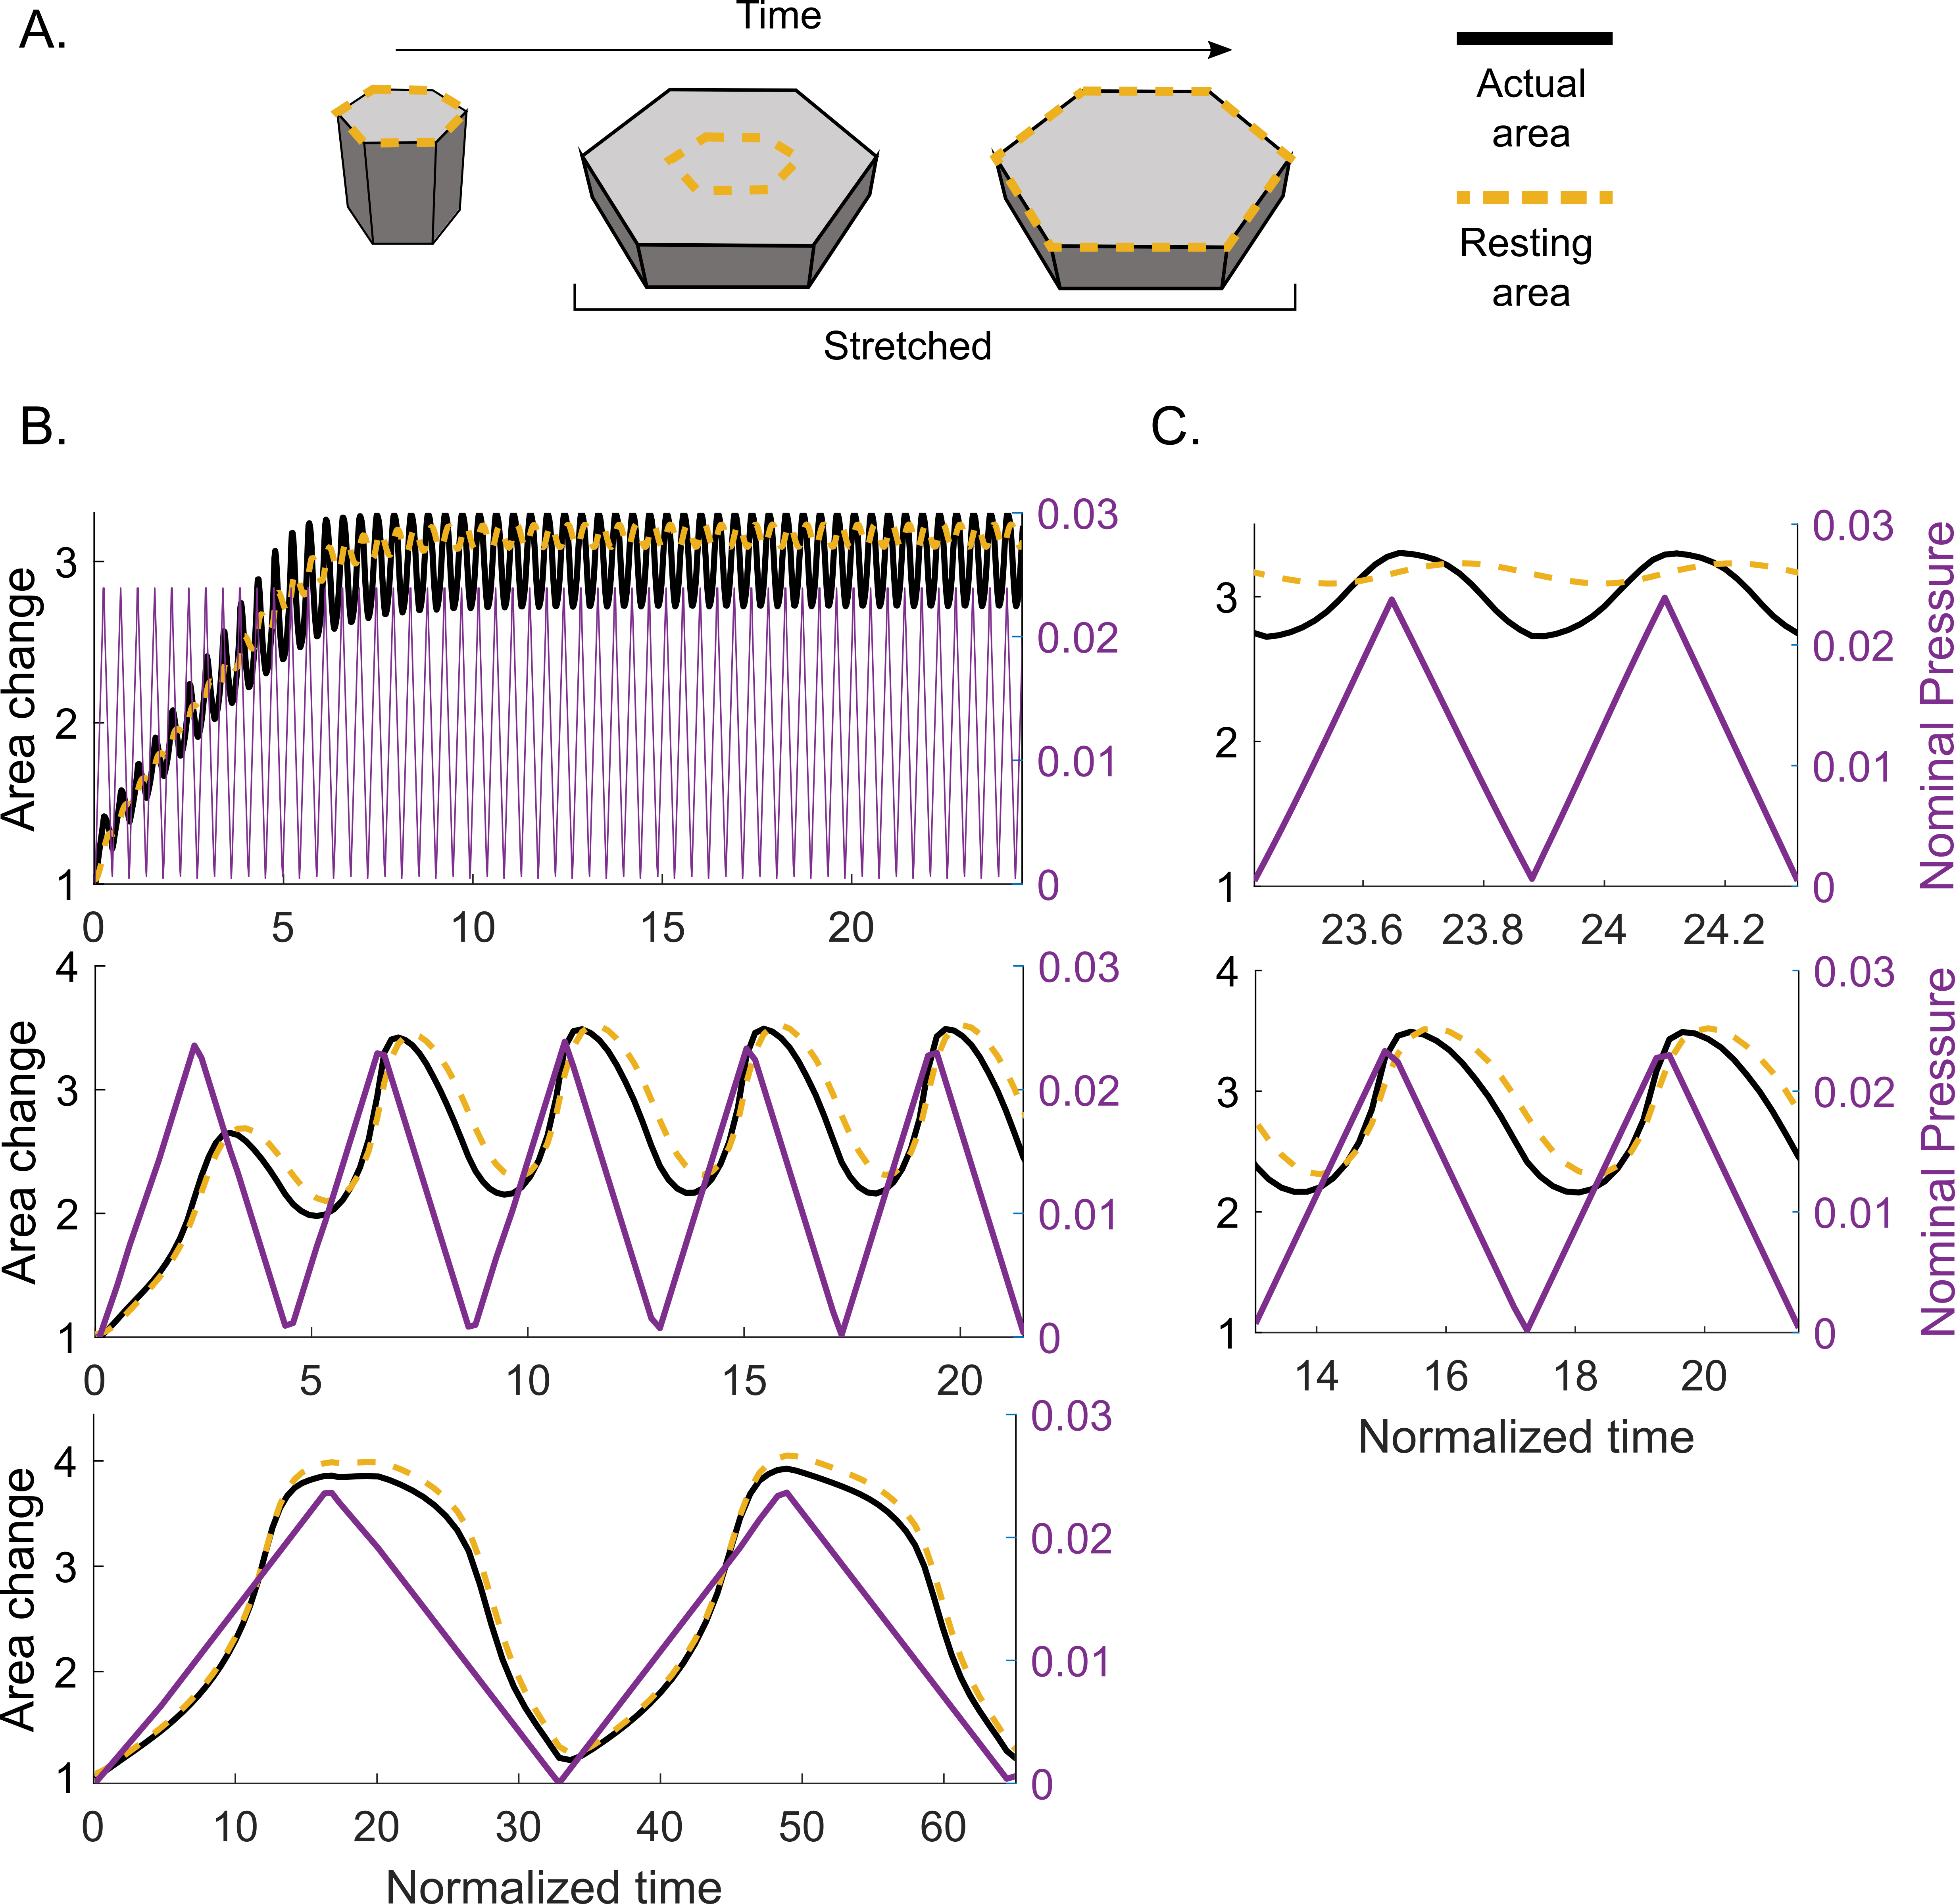
\includegraphics[width=\textwidth]{chap7_area.png}
	\caption{\label{fig_7_7} \textbf{Concept of resting area}: (A) Illustration of a resting and actual are of a cell in a monolayer during stretching. (B) Differences in results of resting and actual area when subjected to different rates of pressure. (C) Inset of the last two cycles.
	}
\end{figure}

We observed that, for the slowest condition, the resting area in the
digital dome almost overlapped with the actual area in the last two
cycles. This is because the pressure is changing very slowly at a rate
of 0.2 Pa/s, allowing the cells sufficient time to remodel and dissipate
elastic stresses. Viscoelastic and turnover timescales in simulations
are around 10-30s, which means that over a period of 2000s, the dome
stretches considerably and returns to original flat state.

However, when pressure is applied more rapidly in cycles of 20s, strains
accumulate because cells are unable to dissipate stored elastic energy
due to insufficient time. The simulations show that the resting area
marginally changes relative to the actual area. Notably, creep
experiments simulations, where tissue is stretched at constant tension,
show strain accumulation at the visco-active timescale, where both
contractility and viscosity are at play.

To sum up, the digital dome model explains the different behaviors of
epithelial tissue depending on the rate at which pressure is applied.
Slower rates allow for cell remodeling and dissipation of elastic
stresses, while faster rates result in strain accumulation due to
insufficient time for dissipation.

\hypertarget{summary}{%
	\section{Summary and Discussion}\label{summary}}

In this study, we investigated the mechanics of epithelial tissue by
applying pressure at varying rates. Initially, we applied a constant
pressure of 200Pa, which led to the dynamic inflation of domes and
eventually reached a steady-state in strain. Due to the spherical
geometry of the tissue, we observed a non-monotonous tension-strain
curve in response to the constant pressure. However, we found that the
true tension-strain curve exhibited increasing tension with respect to
strains at lower values, but at higher strains, the tension appeared to
be independent of the strains.

Furthermore, our results showed that the domes accumulated strain
through the cycles when probed with fast-changing pressure and reached a
steady-state in later cycles. However, when stretched slowly, the domes
stretched to high strains without accumulating strain.

To understand the behavior of epithelial tissue, we developed an active
viscoelastic fluid model, which allowed us to probe the time-dependent
response of the tissue to pressure. Our experimental and computational
framework revealed that the response of the domes to cyclic pressure is
dependent on active viscoelasticity.

The tissue stretches to balance the tissue tension with externally
applied pressure timescale and reaches a steady-state strain by actively
remodeling the cortex. Our digital dome studies indicated that different
timescales play a role together in producing the tissue's response to
pressure. These timescales are the reflection of interplay between
cortical turnover, crosslinkers, and network reorganization allows for
large deformations and rapid shape changes.

We can interpret our model results in terms of a multidimensional
Maxwell model. The classical Maxwell model is composed of a spring and a
dashpot, representing the elastic and viscous elements, respectively. In
this case, we can imagine a similar model with two branches: one with a
spring and dashpot representing the passive viscoelasticity, and a
second branch with an active spring representing the active component.
If the stretching is done slowly, only the dashpot would stretch while
the elastic component (spring) would not. On the other hand, if we
stretch too fast, the viscous component would not move while only the
spring would deform.

Previous research has approached the system in a similar manner, where
epithelial tissue was modeled using viscoelastic models of springs and
dashpots. One particularly interesting model was developed by
Khalilgharibi in 2019, which characterizes the response of a suspended
monolayer to stretch and demonstrates that the dynamics are similar to
that of a single cell, due to the role of the actomyosin cortex. They
used a model with two springs in parallel, one of which can change its
length dynamically. This explains the relaxation of the monolayer, where
the active contractility of the cortex changes the resting length of the
active spring in the model, which closely relates to our ``resting
area'' concept.

Another study found that viscoelastic dissipation could explain the
shortening or elongation of cell junctions in drosophila embryos. They
demonstrated that the dissipation occurs at the minute timescale, at the
same timescale as myosin pulses. It is also interesting that they found
actin turnover plays a key role in this dissipation.

Applying tensions and strains to suspended cells \textit{in vitro} is a
challenging task, and it is important to note that adherent monolayers
may exhibit different behaviors from suspended cells. The tissue matrix
provides additional stiffness and can alter the cytoskeletal structure
of cells, which further complicates the understanding of cell mechanics.
In this thesis, we focus specifically on the actin cortex and short
timescales (minutes).

The timescale of actin remodeling is on the order of tens of seconds,
and we did not observe any cellular rearrangement or division at this
timescale in our system (with rare exceptions). Long-term experiments
were not performed due to suspected involvement of other cytoskeletal
components, such as intermediate filaments. In a study by Latorre et
al., activation of intermediate filaments was observed in extremely
stretched cells (\textgreater300\%), which caused re-stiffening and
prevented the cells from stretching too much. This motivated the strain
limiting mechanism imposed in our model. However, in our experiments, we
did not observe any indication of superelasticity, as all cells were
super-stretched at the same time.

In the next chapter, we will endeavor to apply our understanding of
viscoelasticity to generate radical transformation of domes into various
structures.
